\chapter{Agente de inteligência artificial}\label{cap:agente}
O agente oferece uma forma de consultar informações e solicitar ações do cuidado em linguagem natural. Sua função é complementar o aplicativo, não prescrever, escolher doses ou substituir o responsável pelo tratamento. A execução das solicitações permanece sujeita às regras da API e às permissões do contexto.

\section{Evolução e organização}
A proposta inicial utilizou Microsoft Copilot Studio. O desenvolvimento posterior passou a utilizar Microsoft Foundry, com um agente de conversa e uma configuração separada de teste para ferramentas MCP. Essa evolução alterou o modo de integrar voz, contexto e operações de escrita. \cite{DC_ARTIGO,DC_FOUNDRY}

Na configuração de referência de 3 de novembro de 2026, o aplicativo utilizava o agente de conversa na versão 5, sem MCP. A configuração de teste utilizava \texttt{tcc-agent-mcp-teste} na versão 8. A Figura~\ref{fig:agente_arquitetura} apresenta os dois caminhos. A separação evita atribuir à interface de voz funções disponíveis apenas no ambiente de teste.

\begin{figure}[htbp]
\centering
\caption{Separação entre o assistente do aplicativo e o agente de teste com MCP}\label{fig:agente_arquitetura}
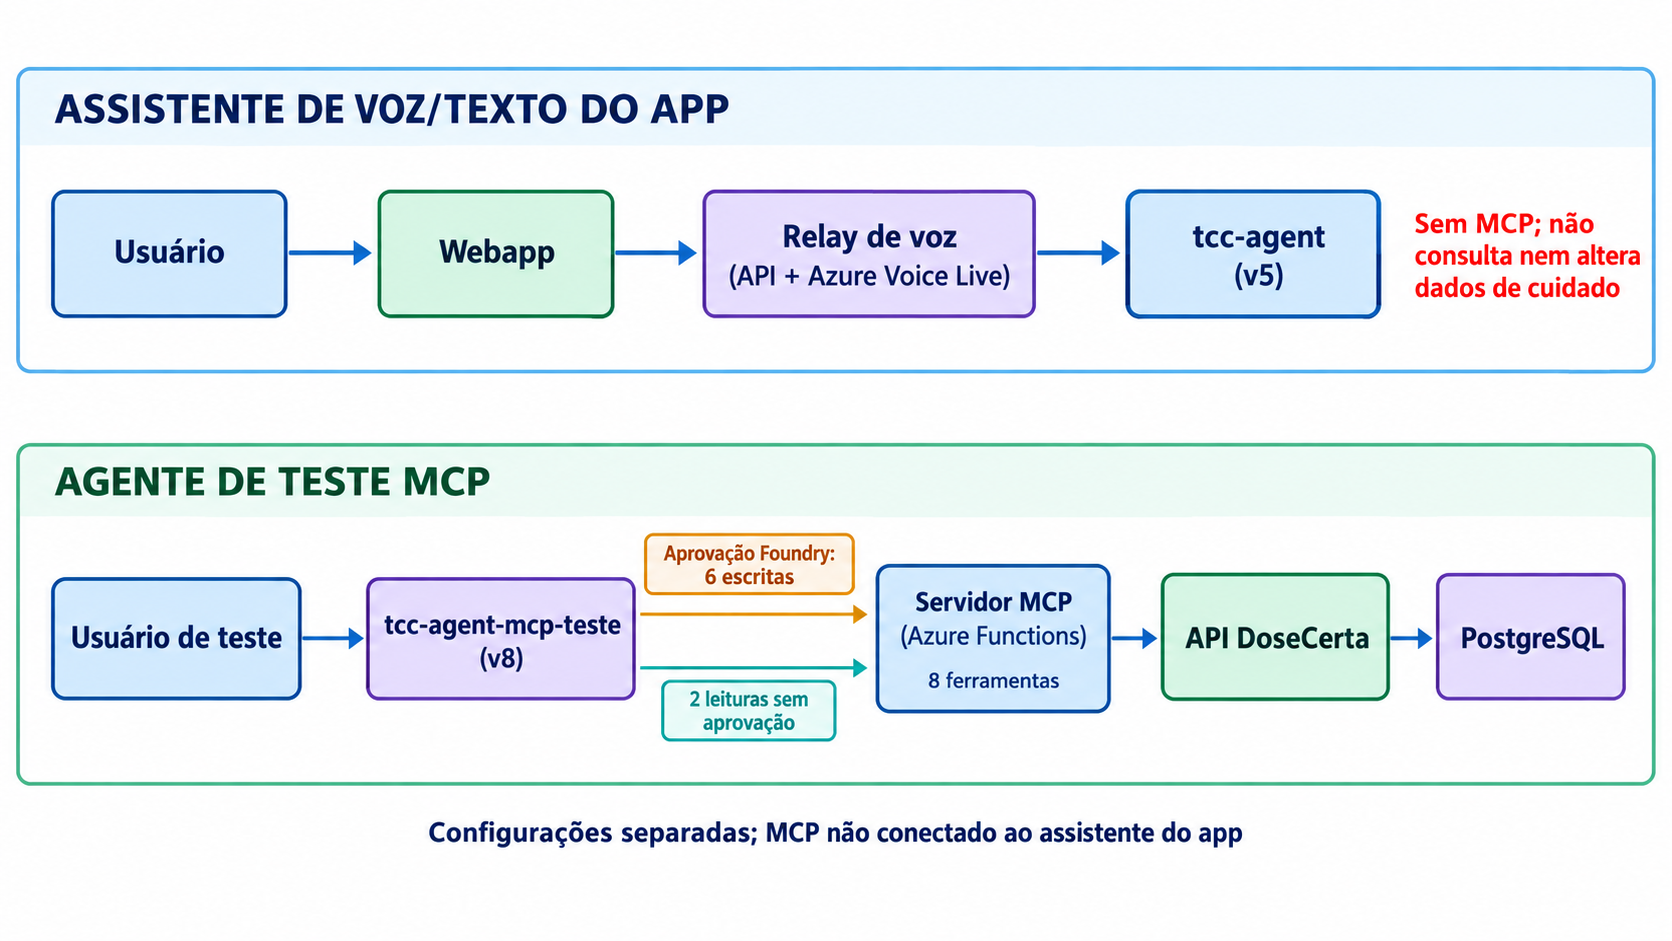
\includegraphics[width=0.98\textwidth,height=0.66\textheight,keepaspectratio]{Figuras/SharePoint/agente_arquitetura.png}
\fonte{Elaboração dos autores. Configuração de referência de 3 nov. 2026.}
\end{figure}


\section{Contexto e recuperação de informações}
Na configuração de referência de 3 de novembro, o agente de conversa utilizava pesquisa em arquivos para recuperar contexto. A utilidade desse recurso depende da seleção, da revisão e da atualização do conteúdo disponibilizado. A existência de um índice não garante que o manual esteja completo ou que os registros atuais do cuidado sejam consultados.

As respostas devem distinguir conhecimento de referência e dados obtidos por ferramenta. Quando uma consulta falha ou retorna informação parcial, o agente precisa informar esse limite antes de afirmar rotina, estoque ou histórico. Textos recuperados são tratados como dados de contexto, não como instruções para alterar a política de operação.

\section{Ferramentas e operações}
A configuração MCP de referência de 3 de novembro reunia duas ferramentas de leitura e seis de escrita. As leituras consultam contexto e registros; as escritas alteram cadastros, rotinas, atividades ou observações. A Tabela~\ref{tab:13-1} apresenta os identificadores da configuração de referência. \cite{DC_FOUNDRY}

{\small\setlength{\tabcolsep}{3pt}\begin{longtable}{p{0.44\textwidth}p{0.12\textwidth}p{0.32\textwidth}}\caption{Ferramentas da cópia MCP do agente, documentadas em novembro}\label{tab:13-1}\\
\hline
\textbf{Ferramenta documental} & \textbf{Tipo} & \textbf{Papel}\\\hline
\endfirsthead\hline
\textbf{Ferramenta documental} & \textbf{Tipo} & \textbf{Papel}\\\hline
\endhead
\texttt{get\_care\_context} & Leitura & Contexto de cuidado\\\hline
\texttt{list\_care\_records} & Leitura & Registros de cuidado e histórico\\\hline
\texttt{create\_medication\_schedule} & Escrita & Criação de rotina\\\hline
\texttt{update\_medication\_schedule} & Escrita & Alteração de rotina\\\hline
\texttt{update\_medication} & Escrita & Alteração de medicamento\\\hline
\texttt{add\_care\_observation} & Escrita & Registro de observação\\\hline
\texttt{create\_daily\_activity} & Escrita & Criação de atividade\\\hline
\texttt{update\_daily\_activity} & Escrita & Alteração de atividade\\\hline
\end{longtable}}{\small\noindent Fonte: Configuração do agente em 3 nov. 2026.\par}

As operações de escrita requerem esclarecimento dos dados necessários e aprovação antes da execução. Uma frase ambígua sobre dosagem ou horário não deve ser convertida diretamente em alteração. A confirmação apresenta a ação e seus argumentos, permitindo ao usuário revisar o pedido.

\section{Aprovação e segurança}
O fluxo da Figura~\ref{fig:agente_aprovacao} começa pela consulta do contexto e pela verificação da clareza do pedido. A negação da aprovação encerra a ação sem escrita. A aprovação, por sua vez, permite prosseguir para o servidor, mas não elimina a validação das regras de negócio e das permissões.

\begin{figure}[htbp]
\centering
\caption{Solicitação, esclarecimento, aprovação e execução de uma operação de escrita}\label{fig:agente_aprovacao}
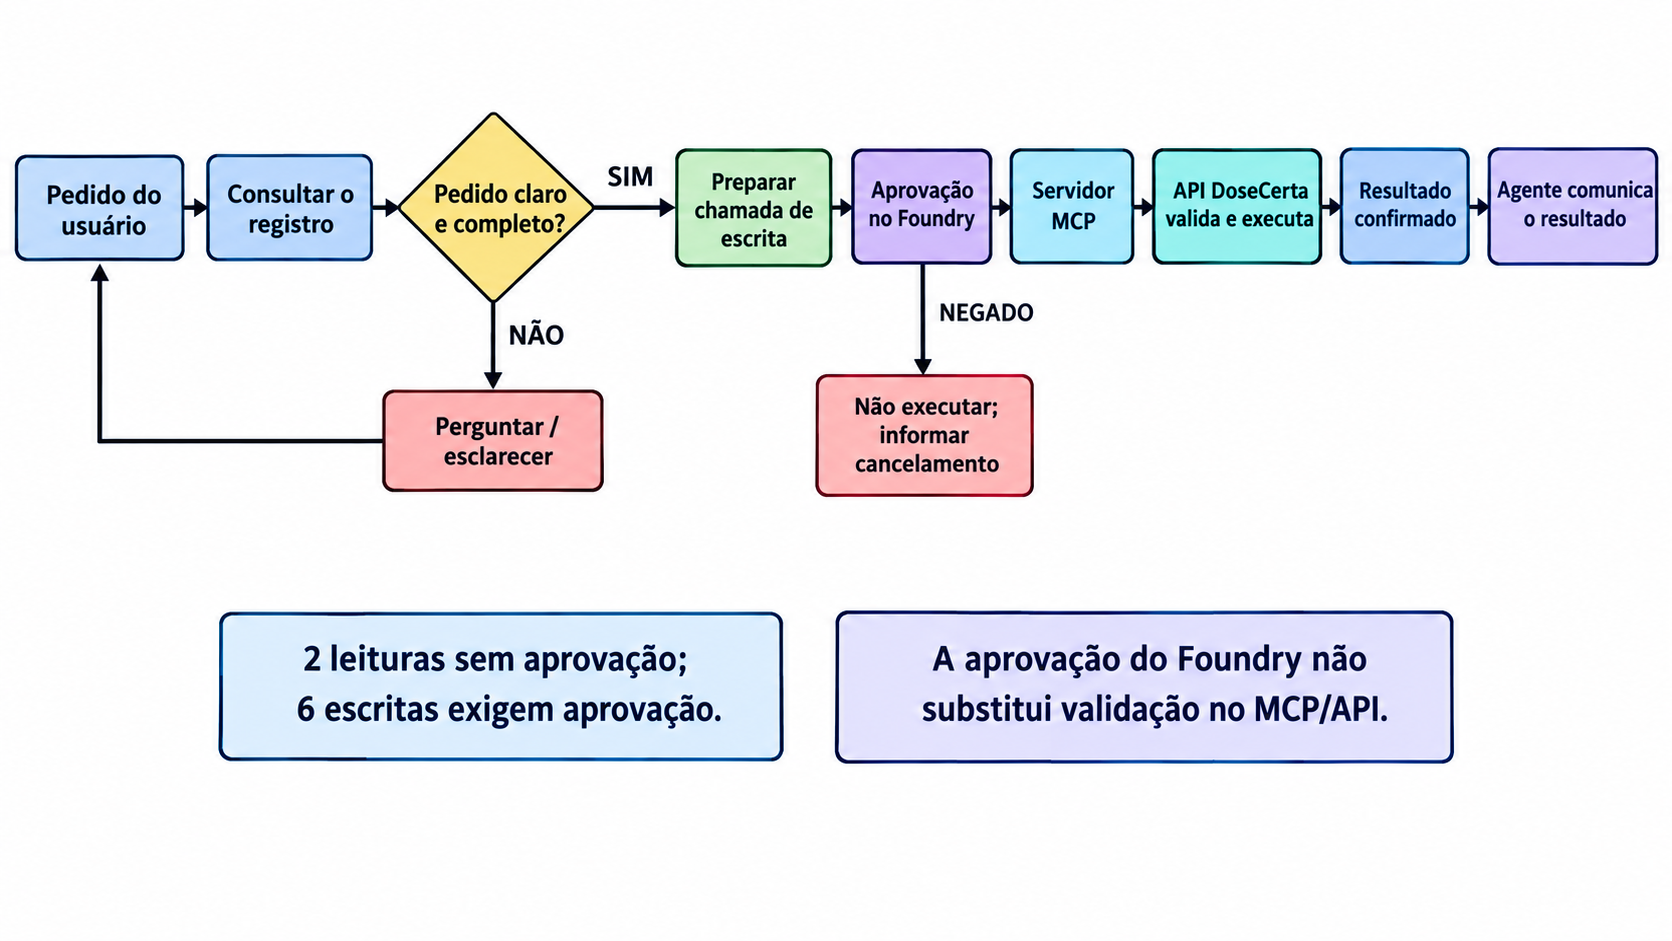
\includegraphics[width=0.98\textwidth,height=0.66\textheight,keepaspectratio]{Figuras/SharePoint/agente_aprovacao.png}
\fonte{Elaboração dos autores (2026).}
\end{figure}


A segurança é distribuída entre identificação do usuário, autorização do serviço e validação na API. Instruções no prompt complementam esses controles, mas não os substituem. Chaves e credenciais não integram o texto nem as capturas públicas.

Quando o retorno de uma ferramenta é incerto, o agente deve consultar o estado antes de solicitar repetição. O mesmo cuidado se aplica à comunicação do resultado: preparar uma chamada, obter aprovação, persistir a alteração e produzir eventual efeito físico são etapas diferentes.

\section{Voz e integração com o Care}
A interface de voz utiliza um relay no backend. Na configuração histórica de 3 de novembro, esse caminho não processa as aprovações exigidas pelas ferramentas MCP, motivo pelo qual foi mantido separado do agente de teste. A resposta conversacional disponível no Care não é, portanto, apresentada como execução automática das oito ferramentas. \cite{DC_FOUNDRY,DC_ANALISE}

A integração deve conservar os caminhos manuais do aplicativo e informar o que foi efetivamente realizado. O agente pode esclarecer uma solicitação, consultar e apresentar um retorno, mas não deve transformar uma falha de acesso em afirmação de ausência de dados.

\section{Avaliação}
A avaliação diferencia recuperação de contexto, escolha da ferramenta, argumentos, confirmação, autorização e efeito persistido. Também considera respostas a ambiguidades, recusa de pedidos clínicos e tratamento de falhas. O teste funcional do servidor MCP avalia uma parte dessa cadeia; não representa, isoladamente, a qualidade do modelo ou da experiência de voz.

Os procedimentos são relacionados à estratégia de integração do capítulo seguinte. Os resultados do agente devem manter a versão, o ambiente e os casos utilizados, permitindo interpretar o alcance de cada evidência.

\section{Estado da integração e alcance da evidência}
Os novos insumos não apresentam uma campanha de interações do modelo que permita estimar precisão de seleção de ferramenta, frequência de falso sucesso ou segurança de escritas em contexto real. A suíte do MCP verifica componentes de software, não corresponde ao mesmo número de conversas avaliadas. A conversa de leitura documentada e a configuração de aprovação são evidências distintas de uma alteração aprovada, persistida e conferida no cuidado correto. \cite{DC_VALIDACAO2026}

A aprovação do Foundry é uma política do caminho do agente, não uma trava universal de toda chamada ao MCP. Quem detiver a chave do serviço pode estar fora desse caminho; por isso, controle de segredo, autorização na API e registro da origem permanecem necessários. A monografia não presume que a integração entre voz, MCP e Care esteja validada apenas porque cada parte responde isoladamente. \cite{DC_VALIDACAO2026}

\section{Relatos posteriores à configuração de referência}
O pacote de novembro relata migração do agente para Azure Voice Live, desligamento do MCP dedicado anterior e consulta somente de leitura ao contexto do paciente por \texttt{GET /v1/care/assistant\_context}; as alterações permaneceriam no aplicativo. Essas informações são relatos de integração de outra frente, não uma atualização confirmada da configuração do agente neste capítulo. Não se apresentam a leitura de receita nem a redução de latência de 94,5 s para 11,0 s como métricas verificadas sem versão, cenário, repetição e registro primário. \cite{DC_VALIDACAO2026}

\section*{\textcolor{DCPendente}{Complementações necessárias}}
\pendencia{AG01}{Confirmar modelo, parâmetros e versões finais do agente publicado e do agente chamado pelo aplicativo. O rótulo interno gpt-5.6-luna precisa de identificação verificável e não deve ser tratado como especificação pública do modelo.}
\pendencia{AG02}{Fornecer evidências das oito ferramentas, aprovação e recusa de escritas, validação do servidor, tratamento de duplicatas e falhas ambíguas. Não executar gravações de teste em dados reais.}
\pendencia{AG03}{Inventariar o conteúdo efetivo do armazenamento vetorial: fontes, revisão, atualização e avaliação da recuperação, incluindo manual atual. Não assumir base atualizada por existir \texttt{file\_search}.}
\pendencia{AG04}{Anexar diálogos sanitizados e registros de chamadas/efeitos persistidos em ambiente de teste; identificar resultado parcial, erro, restauração e limpeza dos dados de teste.}
\pendencia{AG05}{Definir e executar conjunto de avaliação do agente: casos, repetições, referência humana, critérios, falhas clínicas e resultados. Contagens de testes do MCP não são desempenho do modelo.}
\pendencia{AG06}{Documentar permissões, rotação de chaves, limites de acesso, retenção e proteção contra instruções maliciosas em dados. Distinguir controles verificáveis de orientações do prompt.}
\pendencia{AG07}{Reconciliar a configuração histórica de 03/11 com o relato posterior de Voice Live e ferramenta de contexto somente de leitura; identificar versão ativa, protocolo, permissões e evidência no Care antes de afirmar a integração atual.}
